\chapter{On the Bonding of AlH$_2$, SiH and SiH$_3$ Fragments to a Cyclopentadienyl Moiety}
\footnotetext{Partly based on ``Trends in Cyclopentadienyl-Main-Group-Metal Bonding'', \mbox{P. H. M. Budzelaar}, \mbox{J. J. Engelberts} and \mbox{J. H. van Lenthe}, \textit{Organometallics} \textbf{2003}, \textsl{22}, 1562-1576.}
\label{chap_cyclopentadienyl}

\ifthenelse{\boolean{wholethesis}}{\relax}{\begin{center}\textit{Generated on \today\ at \currenttime}\end{center}}

\noindent\textbf{Abstract:} In this chapter the bonding mechanism of three metal hydride moieties, AlH$_2$, SiH and SiH$_3$, to a cyclopentadienyl ring are analyzed with Valence Bond wave functions. In CpAlH$_2$ and CpSiH the metal hydride groups are situated above a C-C bond ($\eta^2$), while the SiH$_3$ group in CpSiH$_3$ is attached to a single C-atom ($\sigma$) and positioned outside the ring. The VB energies and weights of the separate structures, the overlap between the orbitals and the resonance energy contributions indicate that the character of the bond between Cp and the metal hydrides is mainly covalent. For CpAlH$_2$ and CpSiH it is a combination of $\sigma$- and $\pi$-like structural contributions, while for CpSiH$_3$ it is $\sigma$-like only. Besides these covalent contributions in all cases a modest ionic structural contribution is discernible.

\clearpage

\section{Introduction}

The way atoms bind together to form molecules has puzzled scientists over the past centuries. In 1916 Lewis wrote a historic paper about atoms and molecules on which much of today's chemical knowledge, including concepts as the ``covalent bond'' and the ``octet rule'', is based \cite{lewis}. A covalent bond between two atoms is formed when both atoms share one electron to form a pair. Regarding the octet rule Lewis wrote: ``The atom tends to hold an even number of electrons in the [outer] shell, and especially to hold eight electrons, which are normally arranged symmetrically at the eight corners of a cube.'' In 1927 Heitler and London merged the Lewis concept of a bond with quantum mechanics  by spin-coupling the orbitals on two hydrogen atoms, to represent a covalent bond \cite{heitler}. In some molecules bonds cannot be described by the spin-coupling of two orbitals on two atoms, because bonds are not necessarily restricted to two atoms, but can be extended over several atoms, like for example in benzene. A single covalent Kekul\'{e} structure would describe a molecular system with 3 double and 3 single C-C bonds, \textit{i.e.} 1,3,5-cyclohexatriene (see Figure \ref{ch4.fig.cyclohexatriene}, structure (\textbf{a})).
\begin{figure}[hbtp]
\center
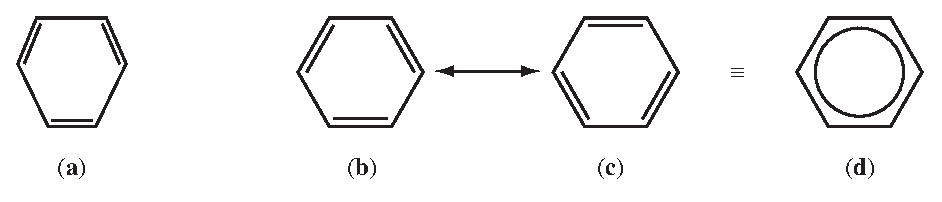
\includegraphics[scale=0.8]{cyclopentadienyl/figures/cyclohexatriene.eps}
\caption{1,3,5-cyclohexatriene (\textbf{a}), the two Kekul\'{e} structures of benzene (\textbf{b} and \textbf{c}) and the structure with delocalized $\pi$ bonds (\textbf{d}).}
\label{ch4.fig.cyclohexatriene}
\end{figure}
The two Kekul\'{e} structures together form the familiar picture with the delocalized $\pi$ electrons. On average, each carbon atom has $1\frac{2}{3}$ bond with each neighboring carbon atom.

Likewise, in organometallic chemistry a single bond between a metal atom and a ligand can be spread out over several ligand atoms. Bonds between metal atoms and ligands are frequently expressed in the hapticity $\eta^x$. The hapto number ($x$) is the number of ligand atoms within bonding distance of the metal \cite{powell}. This sort of bonding is commonly found in metallocenes, which have a sandwich-like structure with a metal atom clamped between two cyclopentadienyl rings. In that case transition metals form a strong, covalent, and symmetric $\eta^{5}$ bond to the cyclopentadienyl (Cp) groups.

In contrast, main group metals show a bewildering variety of bonding arrangements, from symmetric $\eta^{5}$ via various slipped $\eta^{x}$ structures all the way to pure $\sigma$ bonding. In addition $\eta^{x}$ ($x>1$) structures may occur in various bridging modes. There is no single preferred structural type (for a review see \cite{jutzi}). In Figure \ref{ch4.fig.bondarr} the different idealized arrangements are shown. In the $\eta^2$ arrangement the metal atom is above the middle of the C-C bond and bonded to both carbon atoms.
\begin{figure}[ht]
\center
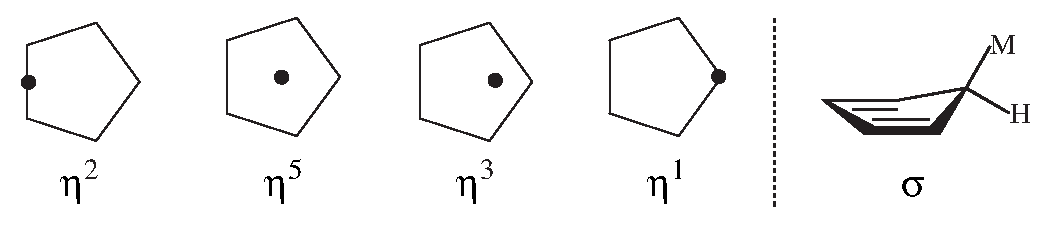
\includegraphics[scale=0.8]{cyclopentadienyl/figures/bondarrangements.eps}
\caption{Idealized representations of Cp-metal bonding arrangements. From left to right $\eta^2$, $\eta^5$, $\eta^3$ and $\eta^1$ hapticities and the $\sigma$ bonding arrangement.}
\label{ch4.fig.bondarr}
\end{figure}
The metal atom is exactly above the middle of the ring in the $\eta^5$ arrangement, having a bond with every carbon. In the $\eta^3$ and $\eta^1$ arrangements the metal atom is located almost at the same location, however, in the $\eta^1$ arrangement the metal atom is exactly positioned above one carbon atom, while in the $\eta^3$ arrangement it is positioned above three carbons. In the representation on the utmost right the metal atom is attached to the cyclopentadienyl ring via a $\sigma$ bond. 

In the transition metal series, the few exceptions to the $\eta^{5}$ bonded situation are easily explained on the basis of the electron-counting rule \cite{shriver}.
% Hoofdstuk 7 met oa "18-electron rule": het anorganische equivalent voor de octet regel van de organici.
For main group metals, no such uniform rule seems to exist. This is illustrated by the series of Cp$_2$M$^{+}$ complexes of the group 13 metals (B, Al, Ga, In and Tl) \cite{macdonald}, where (according to calculations and, in part, confirmed by experiments) on going down the periodic table the structure changes from $\eta^{5}$:$\eta^{1}$ (B; electron precise) to $\eta^{5}$:$\eta^{5}$ (Al; electron excess) back to $\eta^{5}$:$\eta^{1}$ (Ga, In; electron precise) and then to $\eta^{1}$:$\eta^{1}$ (Tl; electron deficient). 
%
% Uitleg electron rich, precise en deficient in Inorganic Chemistry pagina 276
% Diboraan B2H6, je verwacht 14 electronen; heeft er maar 12 --> deficient
%
Several theoretical studies have already been devoted to these half-sandwich and sandwich complexes \cite{kwon}. Ray\'{o}n and Frenking have analyzed the bonding between main group metals (M$^{n+}$) and cyclopentadienyl anion groups ((Cp$^{-}$)$_n$; $n$=1,2) in terms of electrostatic and orbital contributions \cite{rayon}. They concluded that, except for boron, electrostatic interactions dominate the interaction energy and are more important than in the transition metal series.

In this chapter, bonds of main group metal hydrides to a single cyclopentadienyl ring (half-sandwich complexes) will be examined in terms of Lewis structures with Valence Bond (VB) wave functions which are superpositions of covalent and ionic VB structures. From the contribution of each of the structures and their relative energies, the bond type will be derived and a rationalization of the preferred hapticity will be given. 

To analyze this type of bond the first two main group metals with valence electrons in the $p$ orbitals, \textit{i.e.} aluminum and silicon, are selected. To keep the molecules as simple as possible, the metal atoms have been substituted with simple hydrogen atoms. In total, three metal hydrides will be examined: AlH$_2$, SiH and SiH$_3$. 

\section{Methods}

\subsection{\label{ch4.sec.geom}Geometries and Slippage Curves}

To obtain the most favorable position of the metal atom M above the Cp ring in CpAlH$_2$, CpSiH and CpSiH$_3$ the metal hydride moiety is dragged over the ring (the $\eta^2$ geometry and the direction of the slippage are shown in Figure \ref{ch4.fig.slip}).
\begin{figure}[hbtp]
\center
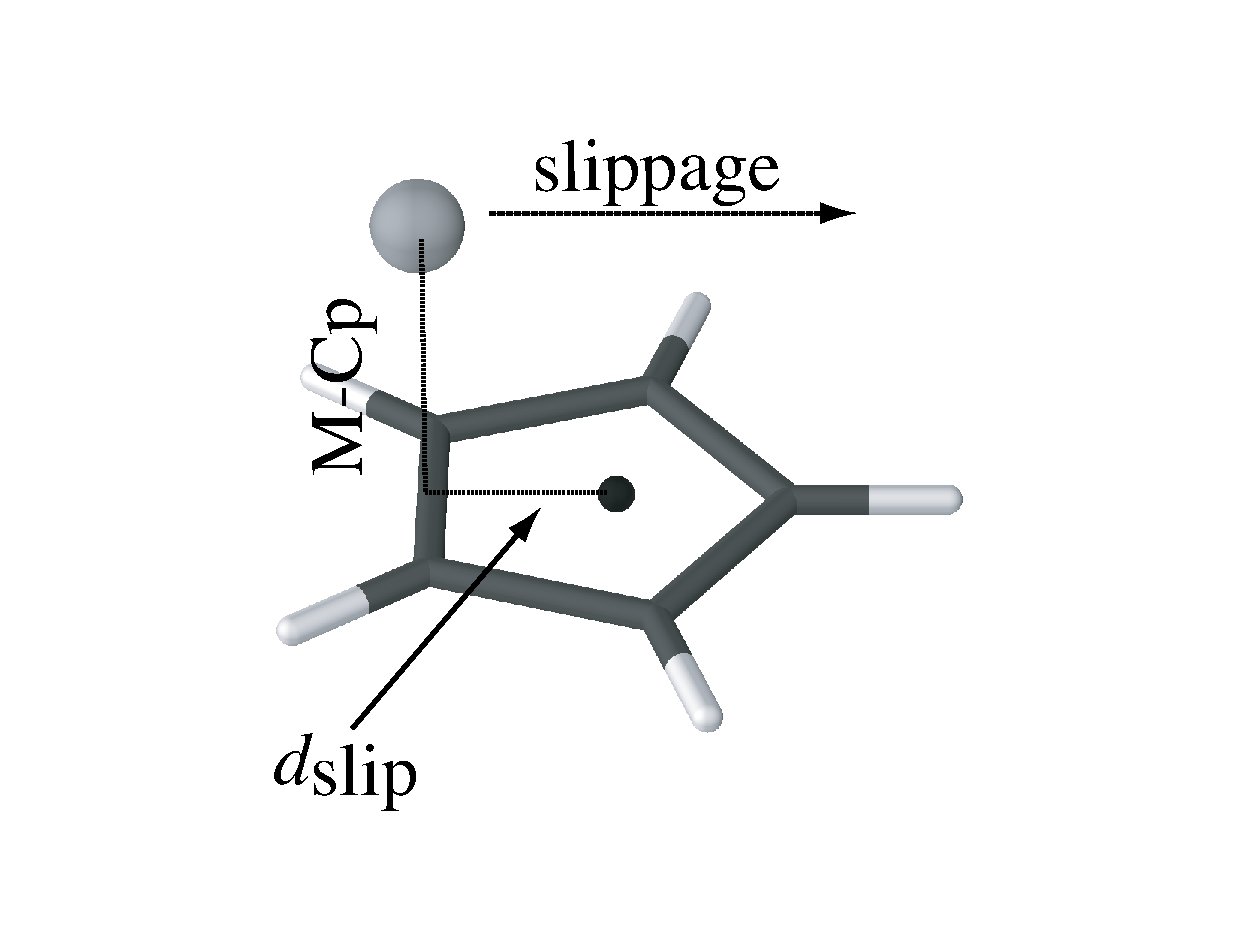
\includegraphics[scale=0.3]{cyclopentadienyl/figures/verloop.eps}
\caption{The metal hydride moiety (sphere) is dragged along a straight line over the ring from above a C-C bond ($\eta^2$; shown here) to the $\sigma$ position outside the ring via the $\eta^5$, $\eta^3$ and $\eta^1$ positions (see Figure \ref{ch4.fig.bondarr}).  $d_\mathrm{slip}$ is the distance of the projection of the metal atom M on the ring to the center of mass (black dot). M--Cp is the distance of the metal atom to the ring.}
\label{ch4.fig.slip}
\end{figure}
At fixed $d_\mathrm{slip}$ intervals of 0.3~\AA\  the geometry is optimized at the B3LYP level \cite{b3,lyp} using GAMESS-UK \cite{gamess} with the \mbox{6-31G*} basis set, maintaining the $C_\mathrm{s}$ symmetry (mirror plane on the lines M-Cp and $d_\mathrm{slip}$). Except for $d_\mathrm{slip}$, all parameters, including M-Cp are optimized. The energy for these geometries are plotted against the $d_\mathrm{slip}$ values (Section \ref{ch4.sec.slippage}). For the points nearest to the minima in the slippage curves, also the $d_\mathrm{slip}$ parameter is relaxed, which results in $C_\mathrm{s}$ constrained minima.

\subsection{Valence Bond Calculations}

On each of these $C_\mathrm{s}$ constrained slippage curve minima (two per compound, as will become clear later on) a Valence Bond (VB) calculation is performed. Hereto a VB wave function ($\Psi$) is constructed as the superposition of covalent and ionic VB structures ($\Phi_i$):
\begin{equation}
\Psi = \sum_{i} c_{i}\Phi{_i}.
\label{ch4.eq.psi}
\end{equation}
Through variational optimization the coefficients ($c$) of these separate VB structures are obtained.
Weights for each structure, which indicate its importance in the wave function, are calculated from the coefficients ($c$) and the overlap between the structures ($S$) with \cite{coulson}:
\begin{equation}
W_{j}=\sum_{i} c_{i}c_{j}S_{ij}.
\label{ch4.eq.weight}
\end{equation}

To investigate the bond between the metal atom and the ring, the VB structures are constructed of two fragments, a metal hydride and a cyclopentadienyl fragment.  Between these two fragments several covalent and ionic bonding arrangements can be defined.

The $\pi$ system of the Cp-fragment contains the molecular orbitals shown in Figure \ref{ch4.fig.cporbs}.
\begin{figure}[htbp]
\center
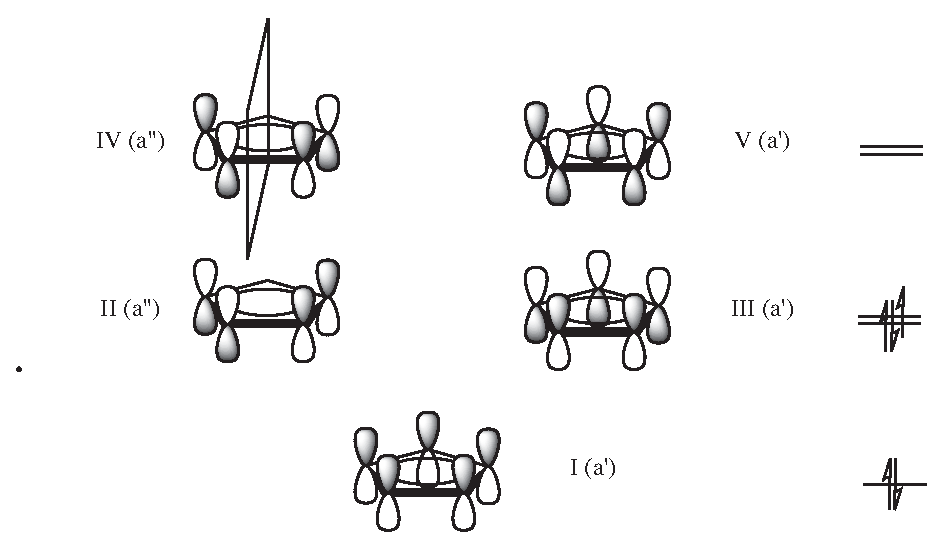
\includegraphics[scale=0.7]{cyclopentadienyl/figures/cp-orbitals.eps}
\caption{The five $\pi$ orbitals of a cyclopentadienyl radical in $C_\mathrm{s}$ symmetry (see mirror plane in orbital IV). Please note that the rings are rotated by 90\degrees\ compared to the model in Figure \ref{ch4.fig.slip}}.
\label{ch4.fig.cporbs}
\end{figure}
Since orbitals II and III are (nearly) degenerate, two electron arrangements are taken into account: in the first arrangement orbitals I and II are doubly occupied, while orbital III (a$^\prime$) is singly occupied. In the second arrangement orbitals I and III are doubly occupied, while orbital II (a$^{\prime\prime}$) is singly occupied. 

All metal hydride fragments have a doublet spin state.\footnote{For SiH$^\bullet$, the quartet has an energy of \mbox{-289.920072} Hartree, while the doublet has an energy of \mbox{-289.988133} Hartree (for more details see \cite{kalemos}). At the B3LYP/6-31G* level of theory, CpSiH has a singlet ground state ($E_\mathrm{s}$=\mbox{-483.551896} and $E_\mathrm{t}$=\mbox{-483.460282} Hartree).} For AlH$_2^\bullet$ and SiH$^\bullet$ there are two possible electron arrangements, one in which an a$^\prime$ $sp^2$-like hybridized orbital is singly occupied and one in which the a$^{\prime\prime}$ $p$ orbital is singly occupied. For SiH$_3^\bullet$ there is only one state: one with an a$^\prime$ $sp^3$ hybridized orbital. 

Two covalent bonds can thus be created by spin-coupling either the singly occupied a$^\prime$ orbitals or the singly occupied a$^{\prime\prime}$ orbitals on both fragments. Spin-coupling the a$^\prime$ orbitals results in the bonding arrangement shown in Figure \ref{ch4.fig.sigma}.
\begin{figure}[htbp]
\center
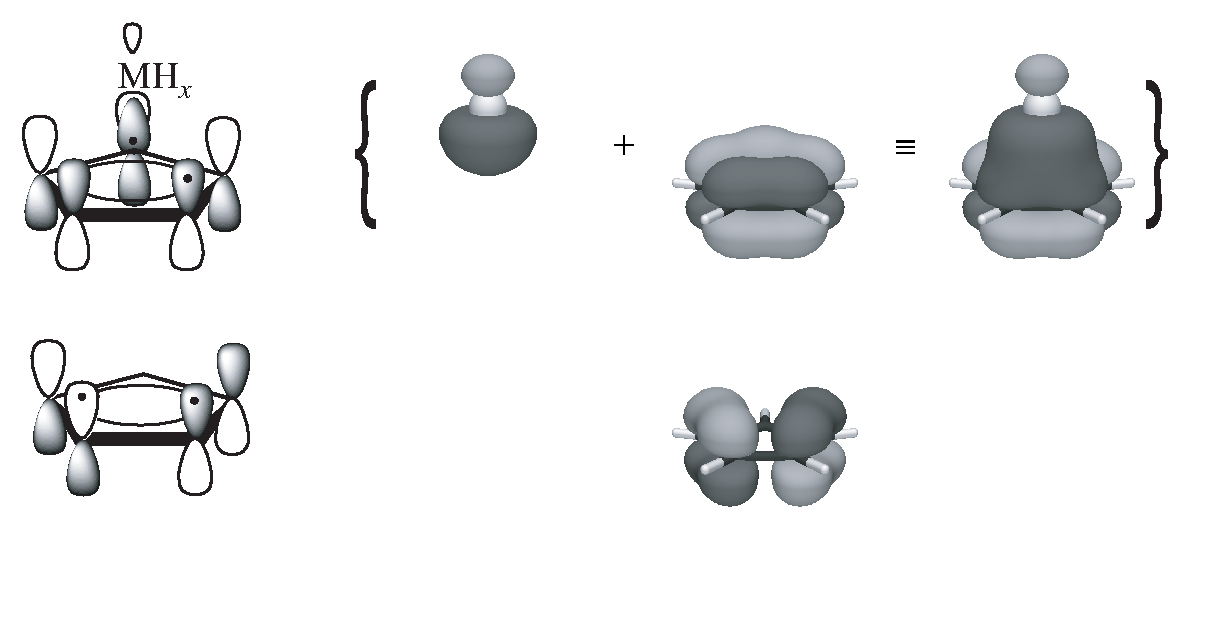
\includegraphics[scale=0.45]{cyclopentadienyl/figures/sigma.eps}
\caption{Schematic representation of the $\sigma$-like bond structure formed by coupling of the singly occupied a$^\prime$ orbitals (top). The a$^{\prime\prime}$ orbital on the Cp-ring is doubly occupied (bottom). Note that the metal hydride moiety is represented as a single sphere.}
\label{ch4.fig.sigma}
\end{figure}
This covalent bonding description will be referred to as a $\sigma$-like bond.

The other bonding arrangement is created by spin-coupling the singly occupied a$^{\prime\prime}$ orbitals on both fragments, \textit{i.e.} the $p$ orbital on the metal hydrides AlH$_{2}^\bullet$ and SiH$^\bullet$ and orbital II on the Cp-ring (Figure \ref{ch4.fig.pi}).
\begin{figure}[htbp]
\center
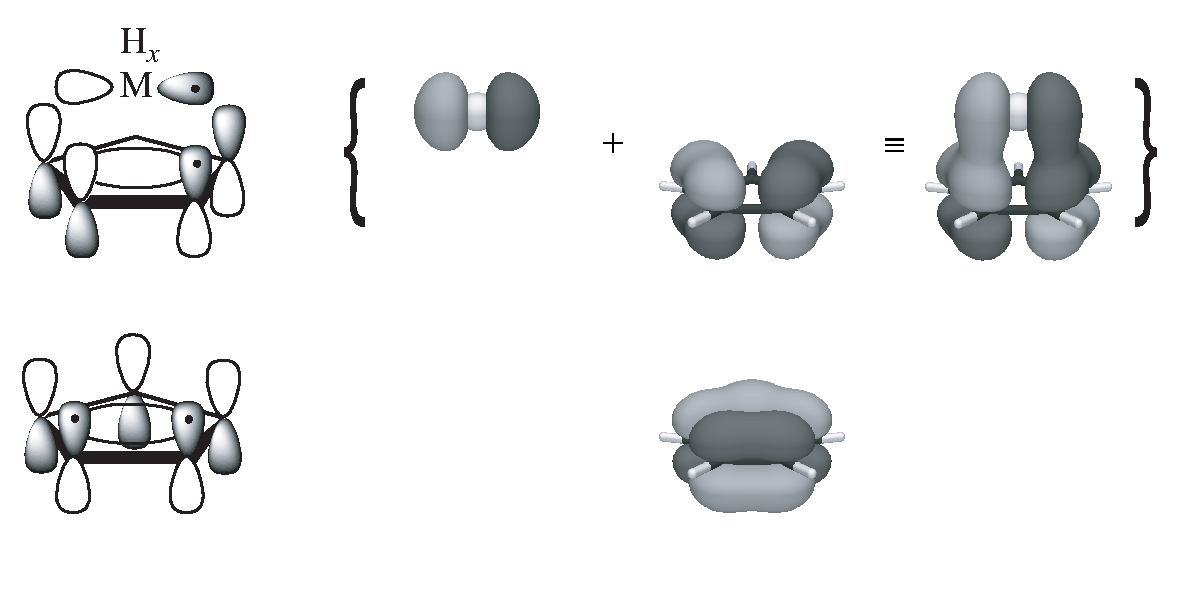
\includegraphics[scale=0.45]{cyclopentadienyl/figures/pi.eps}
\caption{Schematic representation of the $\pi$-like bond structure formed by coupling of the singly occupied a$^{\prime\prime}$ orbitals. The a$^\prime$ orbital on the Cp-ring is doubly occupied (bottom). Note that the metal hydride moiety is represented as a single sphere.}
\label{ch4.fig.pi}
\end{figure}
This second covalent bonding arrangement will be referred to as $\pi$-like bond. Note that the SiH$_{3}^\bullet$ fragment does not possess a suitable a$^{\prime\prime}$ orbital for bonding due to its $sp^3$ hybridization. Therefore, for CpSiH$_3$ only one covalent structure is available.

The other VB structure used for this investigation is ionic in nature, in which the Cp-ring is negatively charged and the metal hydride moiety is positively charged (Figure \ref{ch4.fig.ionic}).
\begin{figure}[htbp]
\center
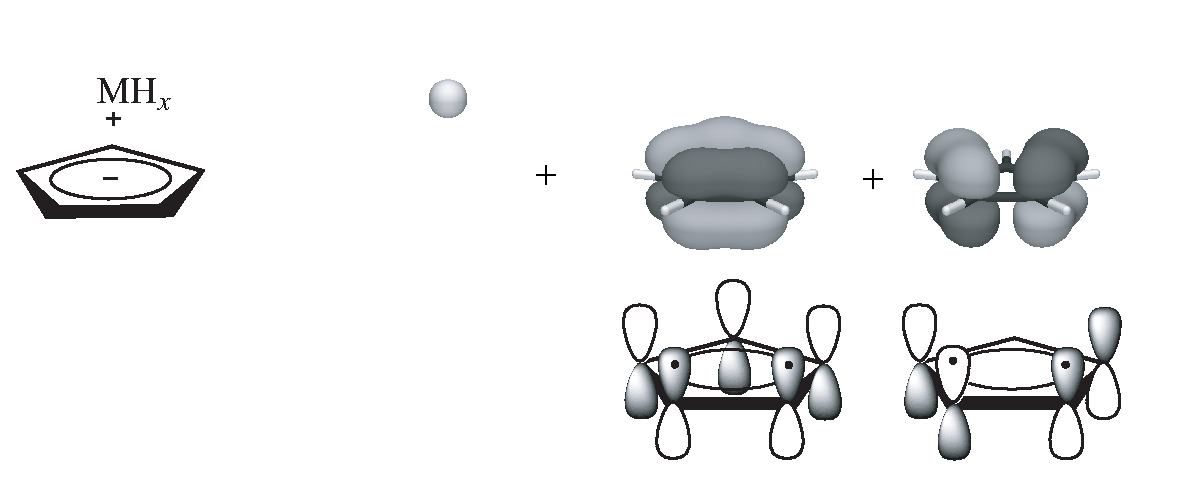
\includegraphics[scale=0.45]{cyclopentadienyl/figures/ionic.eps}
\caption{Schematic representation of the ionic structure formed by doubly occupying both the a$^{\prime}$ and a$^{\prime\prime}$ orbitals on the Cp ring. Note that the positively charged metal hydride moiety is represented as a single sphere.}
\label{ch4.fig.ionic}
\end{figure}
In this situation the Cp-ring contains 6 $\pi$ electrons and is considered aromatic (H\"{u}ckel's rule, $4n+2$ $\pi$ electrons). 

Some initial VB test calculations on another possible ionic structure in which the ring is positively charged (cyclopentadienyl cation; $4n$ $\pi$ electrons, $n$=1; anti-aromatic) and the MH$_x$ group is negatively charged (MH${_x}{^-}$) showed that the VB energy of this structure is higher (\textit{ca.} 0.4 Hartree) than the energies of the other three structures. Therefore, this second type of ionic structure is not included in the subsequent calculations.

For each of the structures described before (Figures \ref{ch4.fig.sigma}-\ref{ch4.fig.ionic}) a separate wave function is constructed, which is separately optimized using the Valence Bond Self-Consistent Field (VBSCF \cite{vbscf1,vbscf2}) method. Orbitals on the separate fragments are kept strictly localized: orbitals on the cyclopentadienyl fragment are not allowed to mix with orbitals on the metal hydride moiety and \textit{vice versa}.

The VB calculations were carried out using the \mbox{TURTLE} program \cite{turtle} as incorporated in the GAMESS-UK package \cite{gamess}. In these studies, the \mbox{6-31G} basis was used for the carbon and hydrogen atoms, while for the main group metal atoms the 6-31G* basis was used. 

Start-up orbitals for the VB structures were created in the following way: 1. For each fragment an RHF calculation was performed and the RHF orbitals were Foster-Boys localized \cite{foster};\footnote{\label{ch4.foot.consequence}As a consequence the orbitals are no longer formally symmetry adapted. However, as will be shown, the deviation is minute.} 2. For each VB structure the appropriate localized fragment orbitals (Figures \ref{ch4.fig.sigma}-\ref{ch4.fig.ionic}) were combined and reoptimized in a single structure VBSCF calculation in which the innershell, the C-H bond and the M-H bond orbitals were kept frozen; 3. The final VB wave function was constructed by the combination of the VBSCF orbitals from the separate single structure calculations. The orbitals were reoptimized in which the innershell, the C-H bond and the M-H bond orbitals were still kept frozen. This type of wave function, in which each structure has its own set of orbitals, is called a Breathing Orbitals Valence Bond (BOVB \cite{bovb1,bovb2}) wave function. 

Following this procedure  for CpAlH$_2$ and CpSiH a three VB structure wave function was obtained (the $\sigma$-like structure (Figure \ref{ch4.fig.sigma}), the $\pi$-like structure (Figure \ref{ch4.fig.pi}) and the ionic structure (Figure \ref{ch4.fig.ionic})). For CpSiH$_3$ a combined wave function of only two structures was used: the $\sigma$-like and the ionic structure.

The contributions of the different structures to the wave function were compared by investigating the weights (see equation \ref{ch4.eq.weight}), the relative energies and the resonance energy ($E_\mathrm{res}$), which is defined as the energy difference between the most stable single structure and the total energy ($E_\mathrm{tot}$) \cite{pauling}. The resonance energy of CpAlH$_2$ and CpSiH can be decomposed in contributions from ionic $\leftrightarrow$ $\sigma$ resonance, ionic $\leftrightarrow$ $\pi$ resonance and $\sigma$ $\leftrightarrow$ $\pi$ resonance by transforming the Hamiltonian matrix ($\mathbf{H}$) to a L\"owdin-orthogonalized \cite{lowdin} structure basis \cite{havenith}. The total VB energy ($E_\mathrm{VB}  = \left < \sum_{i} c_{i}\Phi{_i} | H | \sum_{j} c_{j}\Phi{_j} \right >$) can then be written as:
\begin{equation}
E_\mathrm{VB} = \sum_{i}\sum_{j}c^\prime_{i}c^\prime_{j}H_{ij}^{\bot}=\sum_{i}c^\prime_{i}c^\prime_{i}H_{ii}^{\bot}+\sum_{i}\sum_{j>i}2c^\prime_{i}c^\prime_{j}H_{ij}^{\bot}=\sum_{i}\epsilon_{i}+\sum_{i}\sum_{j>i}\epsilon_{ij},
\label{ch4.eq.energ}
\end{equation}
in which $H_{ij}^{\bot}$ is the L\"owdin-orthogonalized Hamiltonian matrix and the $c^\prime$'s are the structure coefficients in the orthogonalized basis. The energy values ($\epsilon$) are the diagonal elements ($\epsilon_{i}$), which represent the energy contributions of the orthogonalized structures themselves. The off-diagonal elements  ($\epsilon_{ij}$) are the weighted interaction energies between the structures. The sum of the off-diagonal elements is another measure of the total resonance energy ($E^{m}_{res}$), namely with respect to the weighted mean value of the energy of all structures \cite{havenith}.

\section{Results and Discussion}

\subsection{\label{ch4.sec.slippage}Geometry Optimization and Slippage Curves}

In Figures \ref{ch4.fig.slip_cpalh2}, \ref{ch4.fig.slip_cpsih} and \ref{ch4.fig.slip_cpsih3} the slippage curves obtained for CpAlH$_2$, CpSiH and CpSiH$_3$ are shown. The energy relative to the most favorable geometry is plotted as a function of  the slippage ($d_\mathrm{slip}$), which is the distance between the center of gravity of the ring and the  perpendicular projection of the metal atom on the Cp-ring.
\begin{figure}[hbtp]
\center
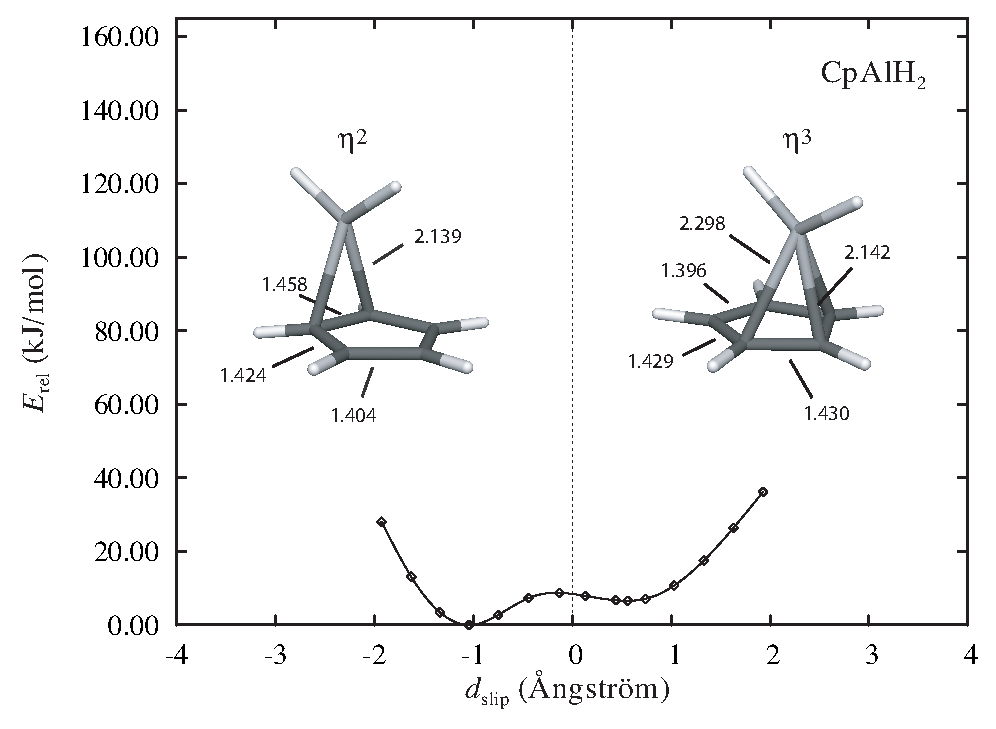
\includegraphics[scale=0.80]{cyclopentadienyl/figures/cpalh2.eps}
\caption{Slippage curve for CpAlH$_2$. For the two minima ($\eta^2$ and $\eta^3$) the corresponding geometries with bonding distances are shown.}
\label{ch4.fig.slip_cpalh2}
\end{figure}
\begin{figure}[htbp]
\center
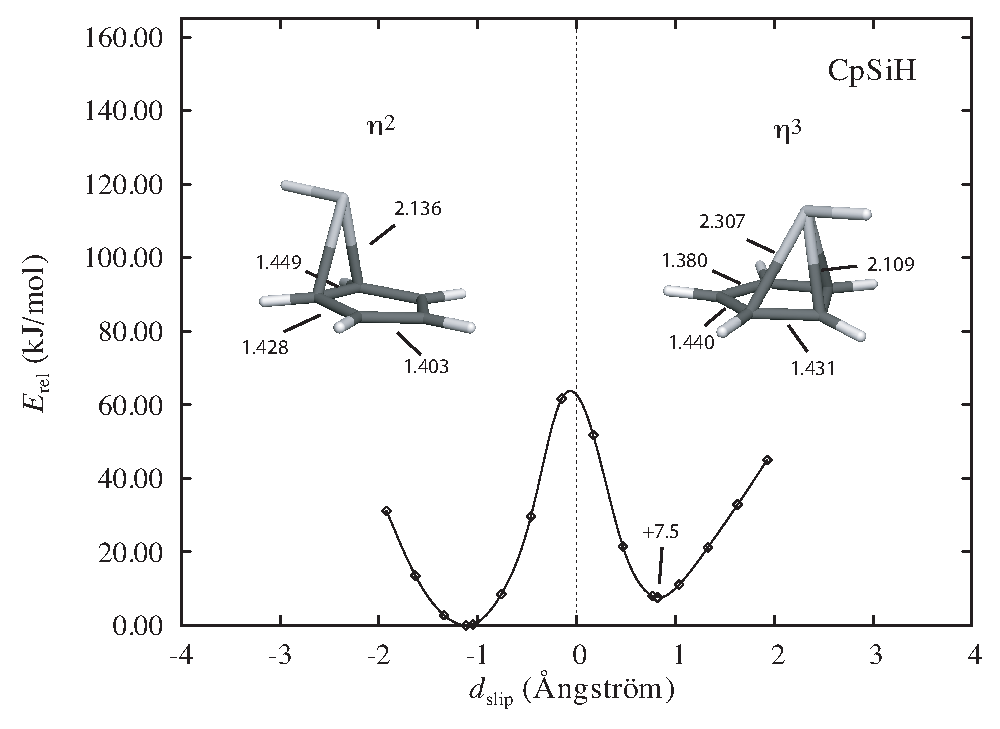
\includegraphics[scale=0.80]{cyclopentadienyl/figures/cpsih.eps}
\caption{Slippage curves for CpSiH. For the two minima ($\eta^2$ and $\eta^3$) the corresponding geometries with bonding distances are shown.}
\label{ch4.fig.slip_cpsih}
\end{figure}
\begin{figure}[hbtp]
\center
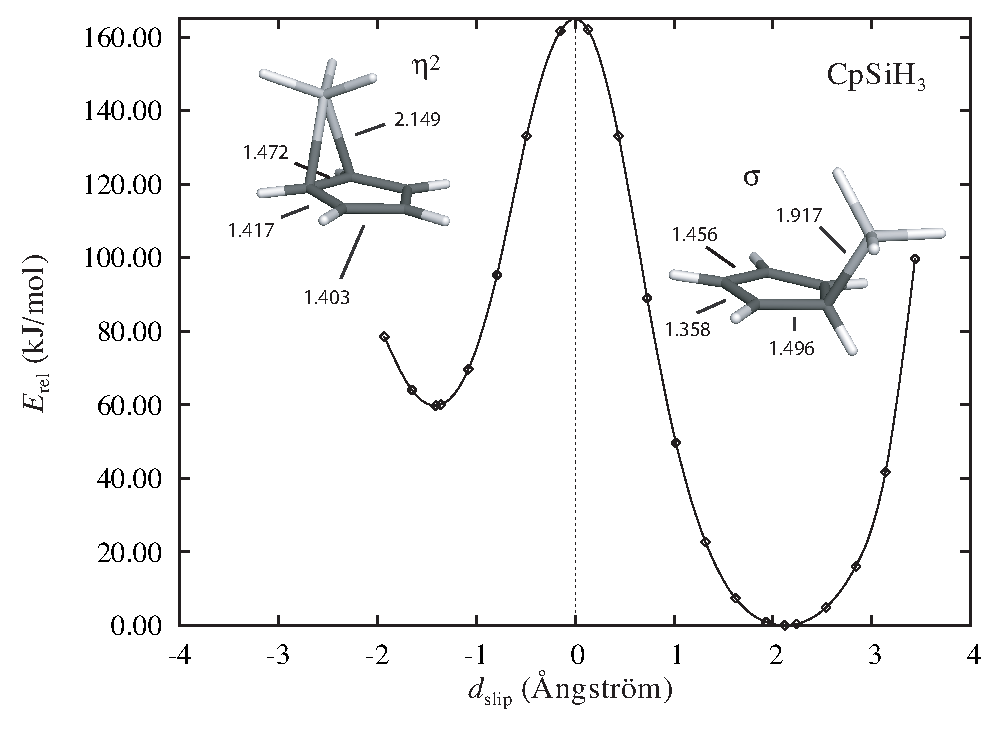
\includegraphics[scale=0.80]{cyclopentadienyl/figures/cpsih3.eps}
\caption{Slippage curves for CpSiH$_3$. For the two minima ($\eta^2$ and $\sigma$) the corresponding geometries with bonding distances are shown.}
\label{ch4.fig.slip_cpsih3}
\end{figure}
At the B3LYP/6-31G* level of theory two stationary points are found for each molecule. Hessian calculations show that the $\eta^2$ geometries of CpAlH$_2$ and CpSiH and the $\sigma$ geometry of CpSiH$_3$ correspond to real minima. The $\eta^3$ geometries of CpAlH$_2$ and CpSiH and the $\eta^2$ geometry of CpSiH$_3$, which all possess only one imaginary frequency, are transition states connecting two equivalent $\eta^2$ geometries on neighboring carbon-carbon bonds in the case of CpAlH$_2$ and CpSiH and two equivalent $\sigma$ geometries on neighboring carbon atoms in the case of CpSiH$_3$. Hessian calculations for the maxima found at the $\eta^5$ positions show two imaginary frequencies for each molecule and are therefore higher order transition states. This means that the slippage curves are no reaction paths and that the metal hydride fragment migrates between the minima ($\eta^2$ for CpAlH$_2$ and CpSiH; $\sigma$ for CpSiH$_3$) along the perimeter of the ring via the ($\eta^3$ for CpAlH$_2$ and CpSiH and $\eta^2$ for CpSiH$_3$) transition states.

Table \ref{ch4.tab.slip} summarizes data obtained from the slippage curves.
\begin{table}[htbp]
\center
\caption{The potential energy with respect to the most favorable geometry, M--Cp, $d_\mathrm{slip}$, the total B3LYP/6-31G* energy and the imaginary frequency (if present) for the two $C_\mathrm{s}$ minima of CpAlH$_2$, CpSiH and CpSiH$_3$.}
\begin{tabular}{|c|c|c|c|c|c|}
\hline
\textbf{Molecule}&
$E_\mathrm{rel}$&
M--Cp&
$d_\mathrm{slip}$&Total B3LYP/6-31G* energy &
$\tilde{\nu}$\\
&(kJ/mol)&(\AA)&(\AA)&(Hartree)& (cm$^{-1}$)\\
\hline
CpAlH$_2$ ($\eta^{2}$) & (0)  & 2.01 & 1.04 & -437.143483 & -\\
CpAlH$_2$ ($\eta^{3}$) & 6.7  & 2.01 & 0.56 & -437.140975 & 93.48$i$ \\
CpSiH ($\eta^{2}$) & (0)  & 2.00 & 1.12 & -483.551896 & -\\
CpSiH ($\eta^{3}$) & 7.5  & 2.00 & 0.82 & -483.548987 & 108.27$i$ \\
CpSiH$_3$ ($\sigma$) & (0)  & 1.74 & 2.12 & -484.793270 & - \\
CpSiH$_3$ ($\eta^{2}$) & 59.8 & 1.97 & 1.41 & -484.770466 & 380.24$i$ \\
\hline
\end{tabular}
\label{ch4.tab.slip}
\end{table}
Both CpSiH and CpAlH$_2$ show a preference of the $\eta^{2}$ geometry over the $\eta^{3}$ geometry. For the transition states, the aluminum atom in CpAlH$_2$ lies closer to the center of gravity (Cg) than the silicon atom of CpSiH, 0.56 \AA\ \textit{vs} 0.82 \AA\ respectively. The bonding distances to the nearest carbon atoms, however, do not differ much, 2.298 \AA\ and 2.142 \AA\ for CpAlH$_2$ \textit{vs} 2.307 \AA\ and 2.109 \AA\ for CpSiH. Therefore, both geometries are denoted as $\eta^{3}$.

While the C-C bonds in CpAlH$_2$ and CpSiH (and CpSiH$_3$ in the $\eta^2$ geometry) are more or less equal (Figures \ref{ch4.fig.slip_cpalh2} and \ref{ch4.fig.slip_cpsih}), the C-C bonds in the $\sigma$ geometry differ more than a tenth of an \AA ngstr\"{o}m (Figure \ref{ch4.fig.slip_cpsih3}). The bond length equilibration in the former two cases is indicative for aromatic behavior: from a geometric point of view, the Cp-rings in CpAlH$_2$ and CpSiH are aromatic, while the Cp-ring in CpSiH$_3$ ($\sigma$ geometry) is not. This is also indicated by the fact that the carbon to which the silicon atom is bonded is $sp^3$ hybridized, which is reflected in the geometric position of the metal atom \textit{outside} the ring ($d_\mathrm{slip}$=2.12 \AA\ ). 

Ray\'on and Frenking have also theoretically analyzed main group metallocenes \cite{rayon}. They found that silicon and aluminum prefer the $\eta^5$ geometry. In the research described here, this geometry corresponds to a second order saddle point (Figures \ref{ch4.fig.slip_cpalh2} - \ref{ch4.fig.slip_cpsih3}). Ray\'on and Frenking, however, considered single metal atoms instead of metal hydride fragments. The hydrogen atoms seem to have a significant influence on the preferred geometry and the bonding. 

\subsection{Valence Bond Calculations}

In Figures \ref{ch4.fig.sihs} and \ref{ch4.fig.sihp} the optimized orbitals that take part in the bonding of CpSiH are shown \cite{molden}. Figure \ref{ch4.fig.sih3} shows the orbitals for CpSiH$_3$. Orbital plots for CpAlH$_2$ are omitted here, since they closely resemble the orbitals of CpSiH. 

\begin{figure} [htbp]
\begin{center}
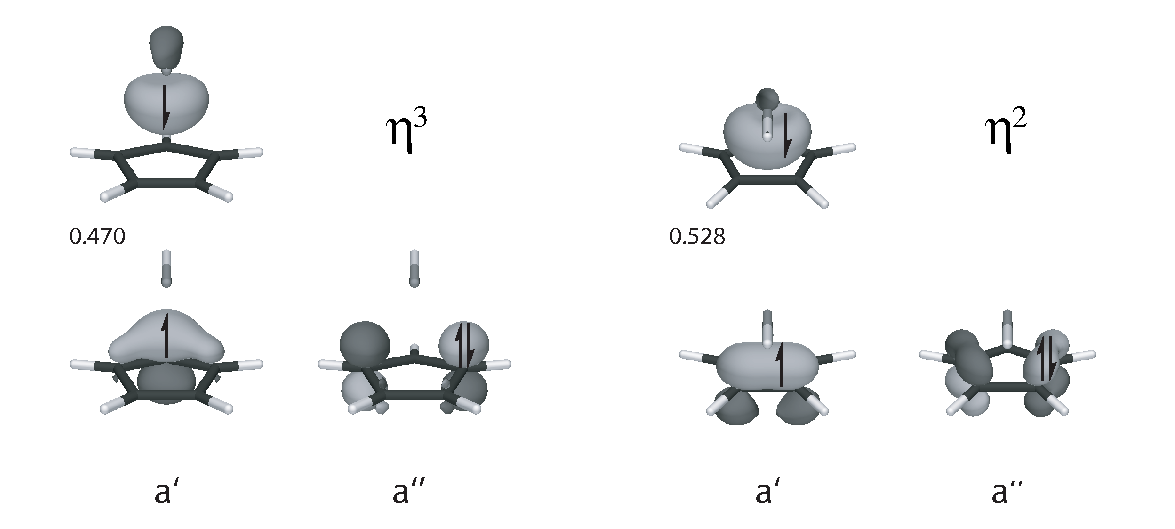
\includegraphics[scale=0.67]{cyclopentadienyl/figures/sih_sigma.eps}
\end{center}
\caption{Contour surfaces (amplitudes -0.1 (light) and 0.1 (dark)) of the two singly occupied spin-paired a$^\prime$ orbitals and the doubly occupied a$^{\prime\prime}$ orbitals for the $\eta^{3}$ (left) and $\eta^{2}$ (right) geometries of CpSiH. The numbers between the singly occupied orbitals are the orbital overlaps. The footnote on page \pageref{ch4.foot.consequence} applies to these VB orbitals.}
\label{ch4.fig.sihs}
\end{figure}

\begin{figure} [htbp]
\begin{center}
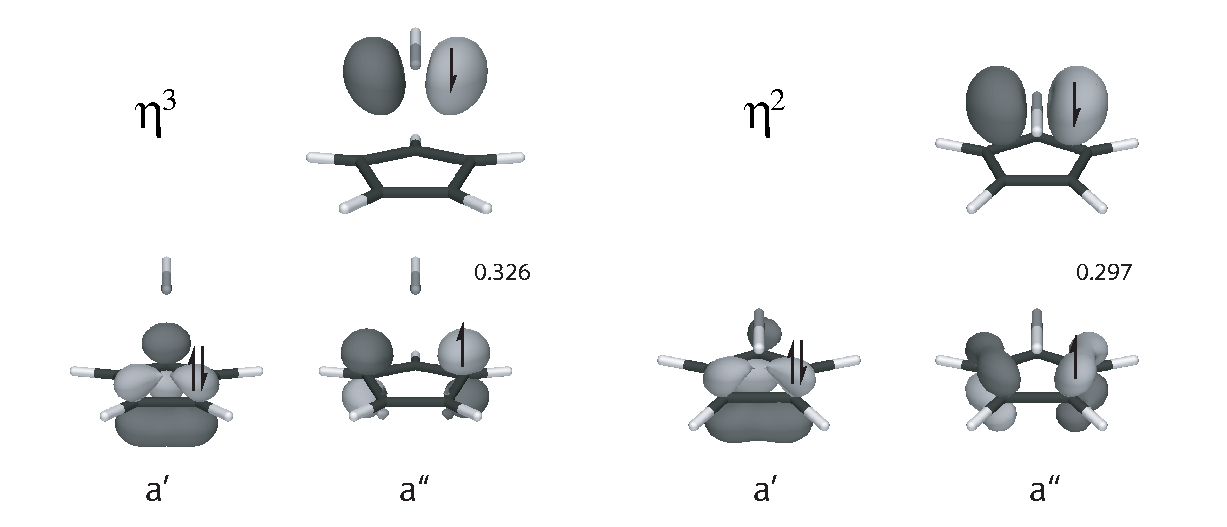
\includegraphics[scale=0.67]{cyclopentadienyl/figures/sih_pi.eps}
\end{center}
\caption{Contour surfaces (amplitudes -0.1 (light) and 0.1 (dark)) of the doubly occupied a$^{\prime}$ orbitals and the two singly occupied spin-paired a$^{\prime\prime}$ orbitals for the $\eta^{3}$ (left) and $\eta^{2}$ (right) geometries of CpSiH. The numbers between the singly occupied orbitals are the orbital overlaps. The footnote on page \pageref{ch4.foot.consequence} applies to these VB orbitals.}
\label{ch4.fig.sihp}
\end{figure}

In Figure \ref{ch4.fig.sihs} the two singly occupied spin-paired a$^\prime$ orbitals on the left form the $\sigma$-like bond description for the $\eta^3$ geometry, the two singly occupied spin-paired a$^\prime$ orbitals on the right form the $\sigma$-like bond description for the $\eta^2$ geometry. The a$^{\prime\prime}$ orbitals are doubly occupied. In contrast, the a$^{\prime\prime}$ orbitals in Figure \ref{ch4.fig.sihp} are singly occupied and spin-coupled in a bond, while the a$^\prime$ orbitals on the Cp-ring are doubly occupied.

The shape of the a$^{\prime\prime}$ orbitals is independent of the occupation (compare the doubly occupied a$^{\prime\prime}$ orbitals in Figure \ref{ch4.fig.sihs} with their  singly occupied equivalents in Figure \ref{ch4.fig.sihp}). In contrast, the a$^\prime$ orbitals are different for both types of occupation, which is most clearly seen when the a$^\prime$ orbitals of the $\eta^3$ geometry are compared. The related a$^\prime$ orbital on the Cp-ring in the $\sigma$ geometry of CpSiH$_3$ (Figure \ref{ch4.fig.sih3}) is directed towards the silicon atom \textit{outside} the ring. This carbon atom in the Cp-ring of CpSiH$_3$ is rehybridized, which can be seen by the position of the hydrogen atom lying below the ring (Figures \ref{ch4.fig.slip_cpsih3} and \ref{ch4.fig.sih3}).

\begin{figure} [htbp]
\begin{center}
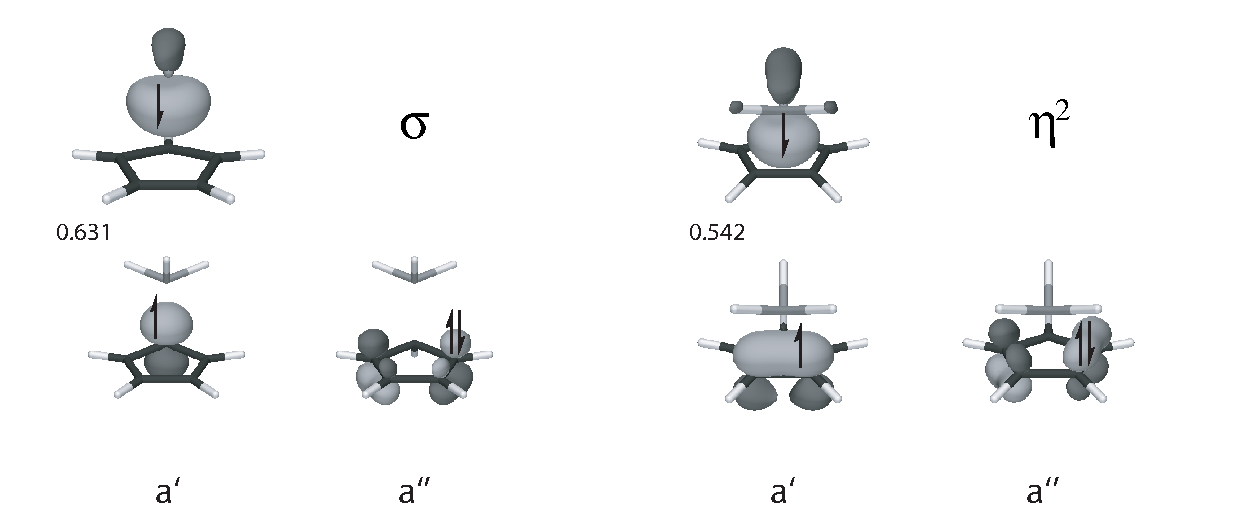
\includegraphics[scale=0.67]{cyclopentadienyl/figures/sih3_sigma.eps}
\end{center}
\caption{Contour surfaces (amplitudes -0.1 (light) and 0.1 (dark)) of the two singly occupied spin-paired a$^\prime$ orbitals and the doubly occupied a$^{\prime\prime}$ orbitals for the $\sigma$ (left) and $\eta^{2}$ (right) geometries of CpSiH$_3$. The numbers between the singly occupied orbitals are the orbital overlaps. The footnote on page \pageref{ch4.foot.consequence} applies to these VB orbitals.}
\label{ch4.fig.sih3}
\end{figure}

The calculated orbital overlap values together with the orbital pictures indicate that covalent bonding occurs in each contributing VB structure. Hence, these structures can be interpreted as ``Lewis''-structures with a $\sigma$ or a $\pi$ bond between the Cp-ring and the metal. In CpSiH the orbitals in the $\sigma$ structure overlap better in the $\eta^2$ geometry than in the $\eta^3$ geometry, 0.528 \textit{vs} 0.470. On the other hand, in the $\pi$ structure the overlap in the $\eta^{3}$ geometry is higher than in the $\eta^{2}$ geometry, 0.326 \textit{vs} 0.297.

As shown in Table \ref{ch4.tab.weights}, the $\sigma$, $\pi$ and ionic structures of CpSiH and CpAlH$_2$ contribute significantly to the VB wave function. Obviously for CpSiH$_3$, only the $\sigma$ and ionic structures contribute. These weights suggest that the Cp-metal bond is a combination of \textit{covalent} and \textit{ionic} character and that the covalent character itself is partly $\sigma$ and partly $\pi$.
\begin{table}[htbp]
\caption{The weights \cite{coulson} of the structures in the VB wave function.}
\center
\begin{tabular}{|c|ccc|}
\hline
\textbf{Molecule}&
\multicolumn{3}{c|}{\textbf{Weights}}\\
&$W_\mathrm{ion}$&
$W_\mathrm{\sigma}$&
$W_\mathrm{\pi}$\\
\hline
CpAlH$_2$ ($\eta^{2}$)&0.30&0.48&0.22\\
CpAlH$_2$ ($\eta^{3}$)&0.31&0.44&0.25\\
CpSiH ($\eta^{2}$)&0.29&0.41&0.30\\
CpSiH ($\eta^{3}$)&0.29&0.38&0.33\\
CpSiH$_3$ ($\sigma$)&0.26&0.74&-\\
CpSiH$_3$ ($\eta^{2}$)&0.34&0.66&-\\
\hline
\end{tabular}
\label{ch4.tab.weights}
\end{table}

Table \ref{ch4.tab.energies} contains the total energy ($E_\mathrm{tot}$), the energy for each separate structure ($E_\mathrm{ion}$, $E_\mathrm{\sigma}$ and $E_\mathrm{\pi}$) in the wave function and the Pauling resonance energy ($E_\mathrm{res}$) \cite{pauling}.
\begin{table}[hbtp]
\caption{The total energy ($E_\mathrm{tot}$) and the energy for each separate structure ($E_\mathrm{ion}$, $E_\mathrm{\sigma}$ and $E_\mathrm{\pi}$), and the resonance energy ($E_\mathrm{res}$), being the energy difference between the most stable single structure and the total energy \cite{pauling}. All energy values are in Hartrees.}
\center
\begin{tabular}{|c|c|ccc|c|}
\hline
\textbf{Molecule}&
\textbf{Total}&
\multicolumn{3}{c|}{\textbf{Structure Energy}}&
\textbf{Resonance}\\
&
$E_\mathrm{tot}$&
$E_\mathrm{ion}$&
$E_\mathrm{\sigma}$&
$E_\mathrm{\pi}$&
$E_\mathrm{res}$\\
\hline
CpAlH$_2$ ($\eta^{2}$)& -435.194422& -435.017811&-435.082625&-434.996217&-0.111797\\
CpAlH$_2$ ($\eta^{3}$)& -435.185474& -435.016456&-435.053468&-434.992522&-0.132006\\
CpSiH ($\eta^{2}$)&-481.590870&-481.403901&-481.451121&-481.438667&-0.139749\\
CpSiH ($\eta^{3}$)&-481.577254&-481.389228&-481.424327&-481.430267&-0.146987\\
CpSiH$_3$ ($\sigma$)&-482.783906&-482.534963&-482.740435&-&-0.043471\\
CpSiH$_3$ ($\eta^{2}$)&-482.726734&-482.545155&-482.661622&-&-0.065112\\ 
\hline
\end{tabular}
\label{ch4.tab.energies}
\end{table}
% Peter --- oorspronkelijk -----
%For both CpAlH$_2$ and CpSiH, the $\pi$ bond structures have almost the same energy for the $\eta^2$ and $\eta^3$ arrangements. Both the ionic and the $\sigma$ bond structures are, however, significantly lower in energy for the $\eta^2$ arrangement. For the ionic structure, this may be due to a closer contact between the fragment and the ring. For the $\sigma$ bond structure, the larger orbital overlap in the $\eta^2$ geometry may contribute; the CpSiH orbital drawings in Figure 12 clearly illustrate the better $\sigma$ overlap in the $\eta^2$ geometry and the better $\pi$ overlap in the $\eta^3$ geometry. For CpAlH$_2$, the ionic structures are intermediate in stability between the $\sigma$ and $\pi$ structures; for CpSiH, the ionic structures are the least stable ones.

For both CpAlH$_2$ and CpSiH, the $\pi$-like bond structures have almost the same energy for the $\eta^{2}$ and $\eta^{3}$ arrangements. The $\sigma$-like bond structures are, however, significantly lower in energy in the $\eta^{2}$ arrangement, than in the $\eta^{3}$ arrangement. This suggests that $\sigma$ type bonding is most important in the $\eta^2$ arrangement. This is also supported by the higher values of $W_\sigma$ for the $\eta^2$ than for the $\eta^3$ arrangement in Table \ref{ch4.tab.weights}. This is probably caused by the larger orbital overlap in the $\eta^2$ geometry: for CpSiH and CpAlH$_2$ it is 0.528 and 0.604 \textit{vs} 0.470 and 0.578 in the $\eta^3$ geometry, respectively. The better overlap is visible in the orbital drawings for CpSiH in Figure \ref{ch4.fig.sihs}: since the orbital on the Cp ring in the $\eta^2$ geometry is more concentrated, \textit{i.e.} spread out over two instead of over three atoms in $\eta^3$, the overlap with the orbital on the metalhydride group is better. While for CpAlH$_2$ the ionic structures are intermediate in stability between the $\sigma$ and $\pi$ structures, for CpSiH the ionic structures are the least stable ones. For CpSiH$_3$ the $\sigma$-like bond structure is \textit{much} more stable than the ionic structure. The $\sigma$-like bond structure is \textit{much} lower in energy for the $\sigma$ arrangement, due to the significantly larger orbital overlap ($\sigma$=0.631 $\eta^2$=0.542; Figure \ref{ch4.fig.sih3}). 

The resonance energies ($E_\mathrm{res}$) of CpAlH$_2$ and CpSiH range from -0.111797 Hartrees for CpAlH$_2$ in the $\eta^2$ geometry to -0.146987 Hartrees for CpSiH in the $\eta^3$ geometry. $E_\mathrm{res}$ values (Table \ref{ch4.tab.energies}) of CpSiH$_3$ are -0.043471 Hartrees ($\sigma$ geometry) and -0.065112 Hartrees ($\eta^2$ geometry). These values are roughly two to three times lower than the other resonance energies of the other geometries. This is in line with expectation: in CpSiH$_3$ there is only a single covalent structure, in the other two cases the covalent character is the combination of $\sigma$ and $\pi$ contributions. This means that neither the $\sigma$ contribution, nor the $\pi$ contribution on their own are representative for the covalent bonding, only the combination is. Therefore, the energy of the separate structures is relatively higher leading to a higher resonance energy.

The decomposition of the resonance energy in contributing resonances of the L\"{o}wdin orthogonalized structures \cite{havenith} is presented in Table \ref{ch4.tab.interactions}.
\begin{table}[htbp]
\caption{The decomposition of the resonance energy in orthogonalized structure contributions ($\epsilon_{ij}$), and the total resonance energy with respect to the weighted mean value of the energy of all structures ($E^m_\mathrm{res}$). All energy values are in Hartrees.}
\center
\begin{tabular}{|c|ccc|c|}
\hline
\textbf{Molecule}&\multicolumn{3}{c|}{$\epsilon_{ij}$}&\\
&ionic-$\sigma$&ionic-$\pi$&$\sigma$-$\pi$&$E^m_\mathrm{res}$\\
\hline
CpAlH$_2$ ($\eta^{2}$)&-0.213347&-0.063315&-0.066387&-0.343049\\
CpAlH$_2$ ($\eta^{3}$)&-0.202372&-0.077936&-0.081104&-0.361412\\
CpSiH ($\eta^{2}$)&-0.170912&-0.065177&-0.064767&-0.300856\\
CpSiH ($\eta^{3}$)&-0.157470&-0.074704&-0.069461&-0.301635\\
\hline
\end{tabular}
\label{ch4.tab.interactions}
\end{table}
For CpAlH$_2$ and CpSiH, the ionic-$\sigma$ interaction is two to three times higher than the ionic-$\pi$ and $\sigma$-$\pi$ interactions. This suggests that the ionic and the $\sigma$ structures separately are not representative for the bonding, but that the combination of the two is. Thus, CpAlH$_2$ and CpSiH possess a polar $\sigma$ bond. Since in the case of CpSiH$_3$ only two structures contribute a decomposition is not necessary. Notwithstanding the large resonance energy in Table \ref{ch4.tab.energies} for CpSiH$_3$ is in line with the ionic-$\sigma$ resonance energy of CpAlH$_2$ and CpSiH. In all cases resonance between the $\pi$ structure with the other two structures is less important.

The difference in minimum geometry between CpSiH$_3$ ($\sigma$) and the other two molecules ($\eta^2$) is rationalized by the absence of a $\pi$-like bond structure in CpSiH$_3$. The extra possibility for CpAlH$_2$ and CpSiH to interact with the cyclopentadienyl moiety via the $\pi$-like bond structure, which has a significant weight (Table \ref{ch4.tab.weights}), structure energy (Table \ref{ch4.tab.energies}) and resonance with the other structures (Table \ref{ch4.tab.interactions}), leads to an enhanced stabilization. In the case that the AlH$_2$ or SiH fragment would occupy the $\sigma$ position, the overlap between the a$^{\prime\prime}$ orbitals would be negligible, and so would be the contribution of that structure.  

\section{Conclusions}

The present work shows that Valence Bond calculations based on three distinct VB structures (Figure \ref{ch4.fig.lewis}), being a superposition of a $\sigma$, a $\pi$ and an ionic structure result in distinguishable differences in the bond types, based on overlap, weight, structure, resonance and interaction energy.
\begin{figure}[htdp]
\begin{center}
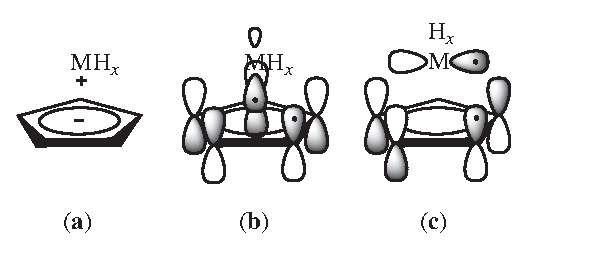
\includegraphics{cyclopentadienyl/figures/lewis.eps}
\end{center}
\caption{The three distinct Lewis structures, the ionic (\textbf{a}), the $\sigma$-like bond (\textbf{b}) and
the $\pi$-like bond (\textbf{c}).}
\label{ch4.fig.lewis}
\end{figure}
The $\sigma$-like bond structure is responsible for the general preference for $\eta^{2}$ geometry, since their energy in the $\eta^2$ geometry is significantly lower than in the $\eta^3$ geometry. Furthermore, the calculations indicate that for CpAlH$_2$ and CpSiH, although $\pi$ bonding is important (reflected in the weights for the $\pi$ structures ($W_\pi$)), it is not the main factor in causing the $\eta^{2}$ geometry, because the energy of the $\pi$ structures is almost equal for the $\eta^3$ and the $\eta^2$ geometry. 

The Hessian calculations for CpAlH$_2$, CpSiH and CpSiH$_3$ indicate that the $\eta^5$ geometry, in which the metal hydride moiety is placed above the middle of the ring, is a higher order saddle point and \textit{not} a transition state. For CpAlH$_2$ and CpSiH the $\eta^3$ geometry is the transition state between two $\eta^2$ minima and for CpSiH$_3$ the $\eta^2$ geometry is the transition state between two $\sigma$ minima.

Our results hold a promise for the study of more elusive main group metal cyclopentadienyl molecules \cite{budzelaar}.

\section*{Acknowledgement}
We would like to thank Peter Budzelaar for his ideas and his work invested in the original review \cite{budzelaar} of which the valence bond section, rewritten in this chapter, was only a small part. We gratefully acknowledge partial financial support from NWO/NCF for use of supercomputer time on TERAS, SARA (The Netherlands, project number SG-032).  

\bibliography{cyclopentadienyl}
\bibliographystyle{../main/achemso}
